% Name: Alarm clock
% Description: A twin-bell alarm clock reading ten past ten, with hour marks, a red second hand, and two little feet.
% Tags: alarm clock, time, clock, illustration

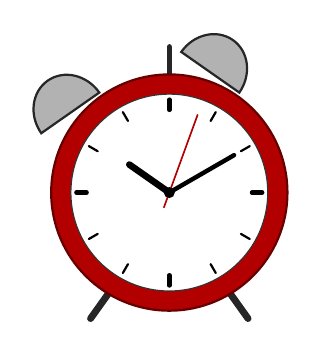
\begin{tikzpicture}[line cap=round]
  % Bells and their hammer
  \foreach \s in {-1,1} \filldraw[fill=gray!60, draw=gray!30!black, thick, rotate around={\s*-35:(0,0)}] (0,1.55) arc (0:180:0.45 and 0.5) -- cycle;
  \draw[gray!30!black, line width=2pt] (0,1.45) -- (0,1.85);
  \draw[gray!30!black, line width=2.5pt] (-0.75,-1.25) -- (-1,-1.6) (0.75,-1.25) -- (1,-1.6);
  \filldraw[fill=red!70!black, draw=red!40!black, thick] (0,0) circle (1.5);
  \filldraw[fill=white, draw=gray!40!black] (0,0) circle (1.25);
  \foreach \h in {1,...,12} \draw[line width={\h==12 || \h==3 || \h==6 || \h==9 ? 1.6pt : 0.8pt}] (90-30*\h:1.05) -- (90-30*\h:1.18);
  % Hands at 10:10: the hour hand a sixth of the way from 10 to 11 (145°), the minute hand on 2 (30°)
  \draw[line width=2.4pt] (0,0) -- (145:0.62);
  \draw[line width=1.6pt] (0,0) -- (30:0.95);
  \draw[red!70!black, line width=0.6pt] (-110:0.2) -- (70:1.05);
  \fill (0,0) circle (0.07);
\end{tikzpicture}
